\documentclass[10pt]{article}

\usepackage{amsmath}
\usepackage{amssymb}
\usepackage{graphicx}
\usepackage[margin=0.75in]{geometry}

\setlength{\parindent}{0pt}
\setlength{\parskip}{4pt}

\begin{document}

\begin{center}
{\Large\textbf{ZMP-Based Stability Cost Formulation}}
\end{center}

\section*{1. Whole-System Dynamics}

The total mass and centre of mass are

\begin{equation}
m=\sum_i m_i,
\qquad
p_C=\frac{1}{m}\sum_i m_i p_{C,i}.
\end{equation}

The angular momentum about the centre of mass is

\begin{equation}
H_C=
\sum_i
\left[
R_iI_i\omega_i^B+
(p_{C,i}-p_C)\times m_i(\dot p_{C,i}-\dot p_C)
\right].
\end{equation}

The total ground force and moment are

\begin{equation}
F=m(\ddot p_C+ge_3),
\qquad
M_O=\dot H_C+p_C\times F.
\end{equation}

\section*{2. Zero-Moment Point}

For a horizontal ground surface,

\begin{equation}
x_Z=-\frac{M_{O,y}}{F_z},
\qquad
y_Z=\frac{M_{O,x}}{F_z},
\qquad F_z>0.
\end{equation}

With $p_C=[x_C,y_C,z_C]^T$,

\begin{equation}
\boxed{
x_Z=
x_C-
\frac{z_Cm\ddot x_C+\dot H_{C,y}}
{m(g+\ddot z_C)}
}
\end{equation}

\begin{equation}
\boxed{
y_Z=
y_C-
\frac{z_Cm\ddot y_C-\dot H_{C,x}}
{m(g+\ddot z_C)}
}.
\end{equation}

\section*{3. Stability Cost}

Let $a$ and $b$ be the half-length and half-width of the support
region. The ZMP constraint with safety margin $\delta$ is

\begin{equation}
|x_Z|\leq a-\delta,
\qquad
|y_Z|\leq b-\delta.
\end{equation}

Define the instantaneous stability cost as

\begin{equation}
\boxed{
L=
\left(\frac{x_Z}{a}\right)^2+
\left(\frac{y_Z}{b}\right)^2
}.
\end{equation}

Thus, $L=0$ at the support centre and increases as the ZMP moves
toward the support boundary.

For $N$ samples, the total stability cost is

\begin{equation}
\boxed{
J=\frac{1}{N}\sum_{k=1}^{N}L_k
}.
\end{equation}

The proposed control input contains the hardware commands:
\begin{equation}
\boxed{
u=
\begin{bmatrix}
a_{\mathrm{ref}}\\
\tau_A\\
\tau_{W,\mathrm{ref}}
\end{bmatrix}
.
}
\end{equation}
Here, $a_{\mathrm{ref}}$ is the linear actuator extension target in metres,
$\tau_A$ contains the arm joint torque commands
in newton-metres, and $\tau_{W,\mathrm{ref}}\in\mathbb{R}^{4}$ contains
the front-left, front-right, back-left, and back-right wheel torque commands
in newton-metres. The lift potentiometer provides position feedback.
The inner actuator controllers convert these commands into the forces and
torques that drive the mechanical system. Wheel torque commands assume
the appropriate CubeMars driver control mode.

The control objective is therefore

\begin{equation}
\boxed{
\min_u J
}
\end{equation}

subject to the ZMP, task, and actuator constraints.

\clearpage
\section*{4. Block Diagram}
\begin{figure}[htbp]
\centering
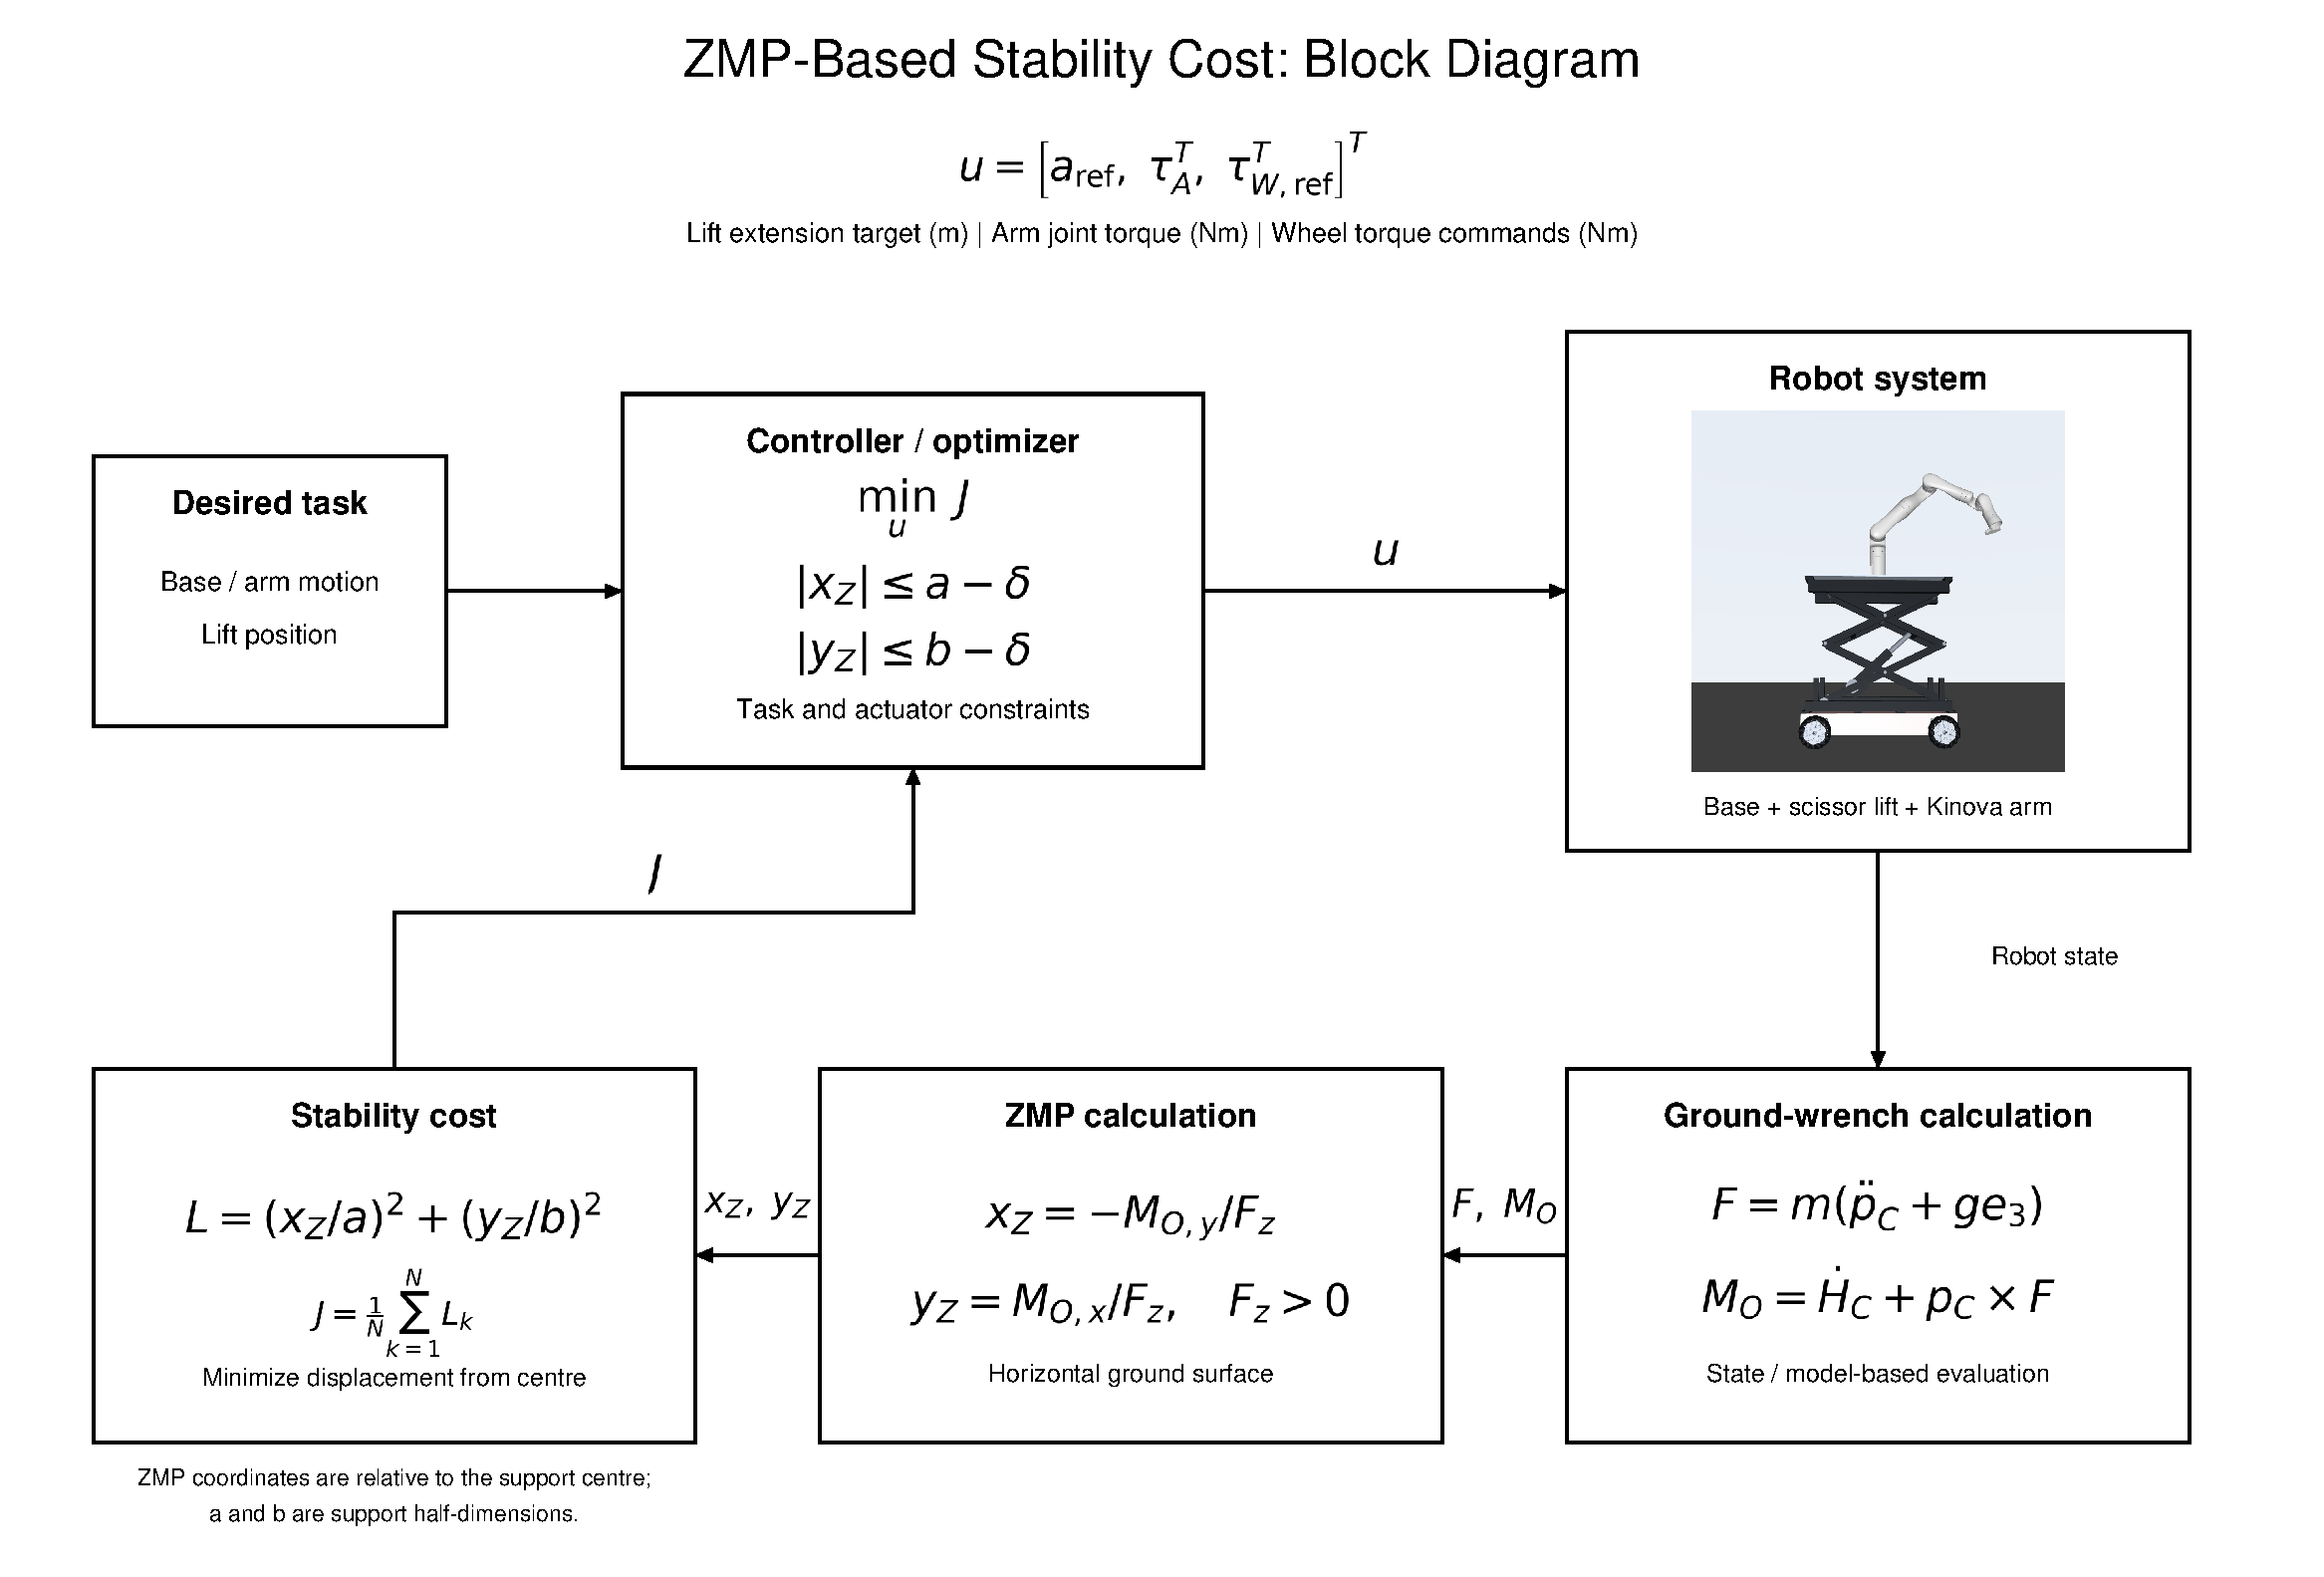
\includegraphics[width=\linewidth]{zmp_final_block_diagram.pdf}
\caption{Block diagram corresponding to the formulation. The controller
selects actuator commands $u$ to minimize $J$ while satisfying the ZMP,
task, and actuator constraints. Robot state and the whole-system model
provide $F$ and $M_O$ for ZMP evaluation. For the cost and rectangular
support constraints, ZMP coordinates are relative to the support centre
with axes aligned with the footprint.}
\end{figure}

\end{document}
